\chapter{Проектирование архитектуры плагина} \label{ch2}
	
% не рекомендуется использовать отдельную section <<введение>> после лета 2020 года
%\section{Введение} \label{ch2:intro}
В данной главе будет проведено проектирование разрабатываемого плагина: будет описана архитектура построения плагинов в Jenkins, а также архитектура разработки, будут выбраны инстркменты разработки, а также расмотрена функциональная модель системы. Поскольку плагин разрабатывается для системы Jenkins, то отладку и тестирование будем проводить в этой системе.

\section{Языки программирования} \label{ch1:sec1}

Для программирования плагина будет использоваться язык Java. Поскольку Jenkis написан на Java, то все плагины необходимо писать на том же языке. Это является главным минусом, а возможно и сложностью при разработке плагинов на Jenkins, поскольку ограничивает свободу разработчика.

Есть возможность разработки плагина с использованием языка программирования Groovy. Groov это динамический язык с возможностями статической типизации и статической компиляции для платформы Java\cite{groovy}, нацеленный на повышение производительности разработчиков, который плавно интегрируется с любой программой Java.

Недостатком такого выбора является то, что абсолютное большинство плагинов написано на чисто Java, а значит сообщества и поддержка при разработке на Java будет значительно большей. Также в сравнии с Groovy, Java обладает большей производительностью\cite{groovyvsjava}, статической типизацией и подходит для разработки приложений в парадигме ООП.

Java — это язык высокого уровня, который можно охарактеризовать следующими словами: объектно-ориентированный, многопоточный, динамический, высокпроизводительный и безопасный \cite{java}. Java используется для разработки высоконагруженный информационных систем, мобильных приложений, плагинов, десктопного ПО и др. К преимуществам Java также можно отнести компилируемость, что обеспечивает высокое быстродействие.

Java будет использоваться для программиования ядра плагина и бизнес-логики. Также для программирования графических компонентов, графиков и диаграмм будет использоваться язык программирования JavaScript. JS - это легковесный, интерпретируемый или JIT-компилируемый, объектно-ориентированный язык \cite{js}, основное предназначение которого выполнять сценарии на веб-страницах, что необходимо при разработке плагина, результаты которого отображаются на веб-страницах.

Помимо прочего, для стилизации компонентов веб-интерфейса будет использоваться язык каскадных таблиц стилей CSS \cite{css}, который позволит настроить удобное отображение и позиционирование элементов на странице плагина Jenkins. 

Верстка страниц будет осуществляться с помощью инструмента Jelly - все разрабатываемые плагины используют данный инструмент в Jenkins, поскольку с ним можно легко интегрировать Java, XML и JS. Jelly — это средство для преобразования XML в исполняемый код, это механизм сценариев и обработки на основе Java и XML \cite{jelly}. В Jelly можно вызывать функции Java, использовать такие синтакситеские конструкции, как циклы, условия и переменные, также он позволяет легко обратиться к объектам в Java.

\section{Инструменты сборки} \label{ch1:sec2}

В качетве инструмента сборки проекта был выбран Maven, который можно использовать для создания и управления любым проектом на основе Java. Maven решает несколько проблем \cite{maven}:

\begin{itemize}
	\item  упрощение процесса сборки;
	\item обеспечение единой системы сборки;
	\item предоставление информации о проекте;
	\item упрощение работы с зависимостями, включая их автоматоическое обновление.
\end{itemize}

Абсолютное большинство разработанных плагинов для Jenkins использует Maven, поскольку Maven предоставляет удобные архетипы для начала разработки плагинов, что делает использование того же Gradle не рациональным.

\section{Библиотеки} \label{ch1:sec3}

Поскольку проект предполагает использовани графиков и диагармм, то необходимо было выбрать инструмент для работы с графиками в Jenkins и Java, который позволит отображать графики прямо на странице задания Jenkins. В качестве этого иструмента была выбрана библиотека Chart.js, которая на данный момент является самой популярной JavaScript библеотекой по оценкам GitHub и загрузок npm \cite{chartjs}. К преимуществам данной библиотеки можно отнести: 
\begin{itemize}
	\item у Chart.js очень подробная документация;
	\item отрисовка canvas делает Chart.js очень производительным, особенно для больших наборов данных и сложных визуализаций;
	\item строит отзывчивый интерфейс - перерисовывает диаграммы при изменении размера окна для идеальной детализации масштаба.
\end{itemize}

\section{Архтектура Jenkins} \label{ch1:sec4}

Перед объяснением построения архитектуры плагинов Jenkins, необходимо привести схему архитектуры Jenkins, где будет отображено место разрабатываемых плагинов в CI системе (рисунок 2.1). Установленные плагины Jenkins-CI, а также локальные сценарии и приложения выполняются на сервере Jenkins-CI и предоставляют расширяемый набор функций управления и обработки данных \cite{article}.

\begin{figure}[ht!] 
	\center
	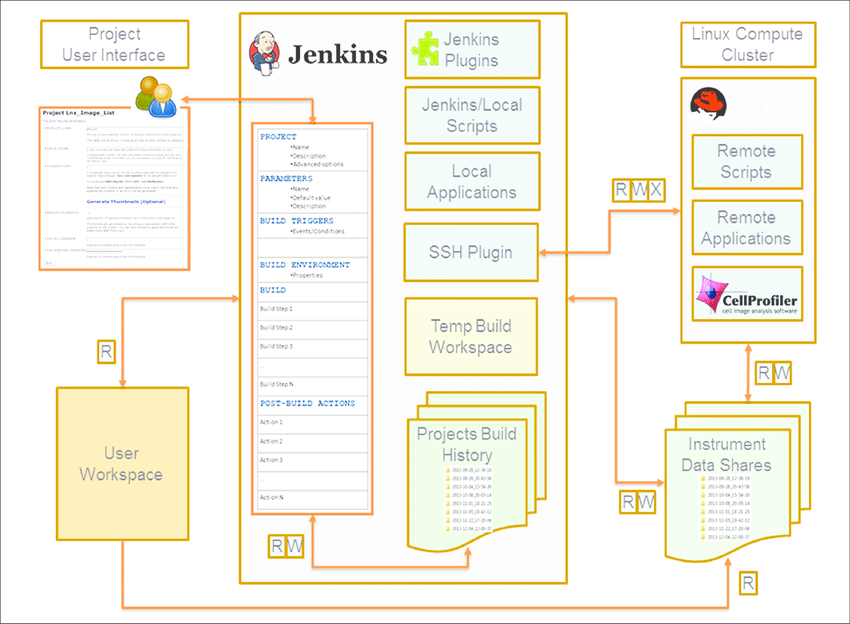
\includegraphics [scale=0.47] {my_folder/images//ArchitectureJenkins}
	\caption{Архитектура Jenkins} 
	\label{fig:ArchitectureJenkins}  
\end{figure}


Архитектура плагинов использует точки расширения, которые, предоставляют разработчикам плагинов возможности реализации для расширения функциональности системы Jenkins \cite{atchplugin}. Точки расширения автоматически обнаруживаются Jenkins во время загрузки системы.

В разрабатываемомом плагине реализация будет происходить через класс Action. Actions являются основным строительным блоком расширяемости в Jenkins: их можно прикреплять ко многим объектам модели, хранить вместе с ними и при необходимости добавлять в их пользовательский интерфейс.

Помимо класса Action для того чтобы создать временные действия, которые будут прикреплены к заданию Jenkins будет использован класс TransientActionFactory, который позволяет создавать действия, которые будут отображаться на страницах Jenkins только при наличии соответствующего объекта - задания.

Разработка будет выполняться в объектно-ориентированной парадигме, т.е. приложение будет разбито на классы, будет применяться наследование, полиморфизм и инкапсуляция. Все классы, которые будут разработаны для плагина описаны в приложении П1.1. При рассмотрении диаграммы необходимо отметить, что два класса являются встроенными в Jenkins, это TransientActionFactoryб который позволяет добавлять действия к любому типу объекта, а также интерфейс Action - добавленный к объекту модели, создает дополнительное подпространство URL-адресов под родительским объектом модели, через которое он может взаимодействовать с пользователями. Actions также способны открывать доступ к левому меню в интерфейсы Jenkins, по которому обычно производится навигация при конфигурировании сборки. Для удобства использования плагина, предполагается добавить дополнительную ссылку в меню слева, для перехода на страницу визуализации метрик, а также динамически обновлять страницу при изменении параметров и фильтров, что и обосновывает использование данных встроенных классов.

Основная часть остальных классов требуется для работы с определенной метрикой статистики выполнения сборок Jenkins, что следует из их названия. Также будет разработан дополнительный класс DateTimeHandler, который позволит создать методы для удобной работы с датой и временем, что необходимо поскольку будет производиться преобразования одних типов дат к другим, сравнение дат между собой, а также получение определенных частей дат.

Функциональная модель в нотации Idef0 отображена в приложении П2.1.-3. Основное внимание на диаграмме уделяется визуализации статистики сборок, поскольку это изначально является целью разработки. Также там будут отражены дополнительные функции такие как фильтрация.

Диаграмма вариантов использования, показывающая функционал плагина отображена в приложении П3.1. На данной диаграмме основное внимание также уделяется процессу визуализации статистики метрик сборок. Основное действующее лицо одно - это пользователь системы, который запускает сборки и работает в CI системе, это может быть любой участник команды, который задействован в разработке, тестировании, доставке и внедрению приложения. В данном случае все эти роли представлены на диаграмме как разработчик.




%% Вспомогательные команды - Additional commands
%
%\newpage % принудительное начало с новой страницы, использовать только в конце раздела
%\clearpage % осуществляется пакетом <<placeins>> в пределах секций
%\newpage\leavevmode\thispagestyle{empty}\newpage % 100 % начало новой страницы